
\begin{minipage}{0.90\textwidth}
\begin{centering}
\wl
\textbf{
    \Large{\reporttype}\\
    \large{\rev- \release}\\
}
\end{centering}
\end{minipage}

    


\section*{First Startup}
The steps presented below will allow the user to setup the filter swapping automation to its factory setpoints.\\

Step 1: Install new bag filter in both housings.\\

Step 2: In the instruments page of the HMI, put FV503A and FV503B in manual mode; activate FV503A only. Ensure that FV407 and FV701 are not activated. Then, manually activate P503.\\

Step 3: Manually adjust the pressure release valve to 20 psi using the pressure indicator near PT503. The pressure release valve is located on the process water manifold and you should find a pressure indicator near the pressure release valve. Before turning the screw, make sure to loosen the locking nut at the base of the screw. To increase the pressure, turn the screw clockwise; to reduce it, turn the screw counter clockwise.\\

\begin{figure}[H]
        \centering
        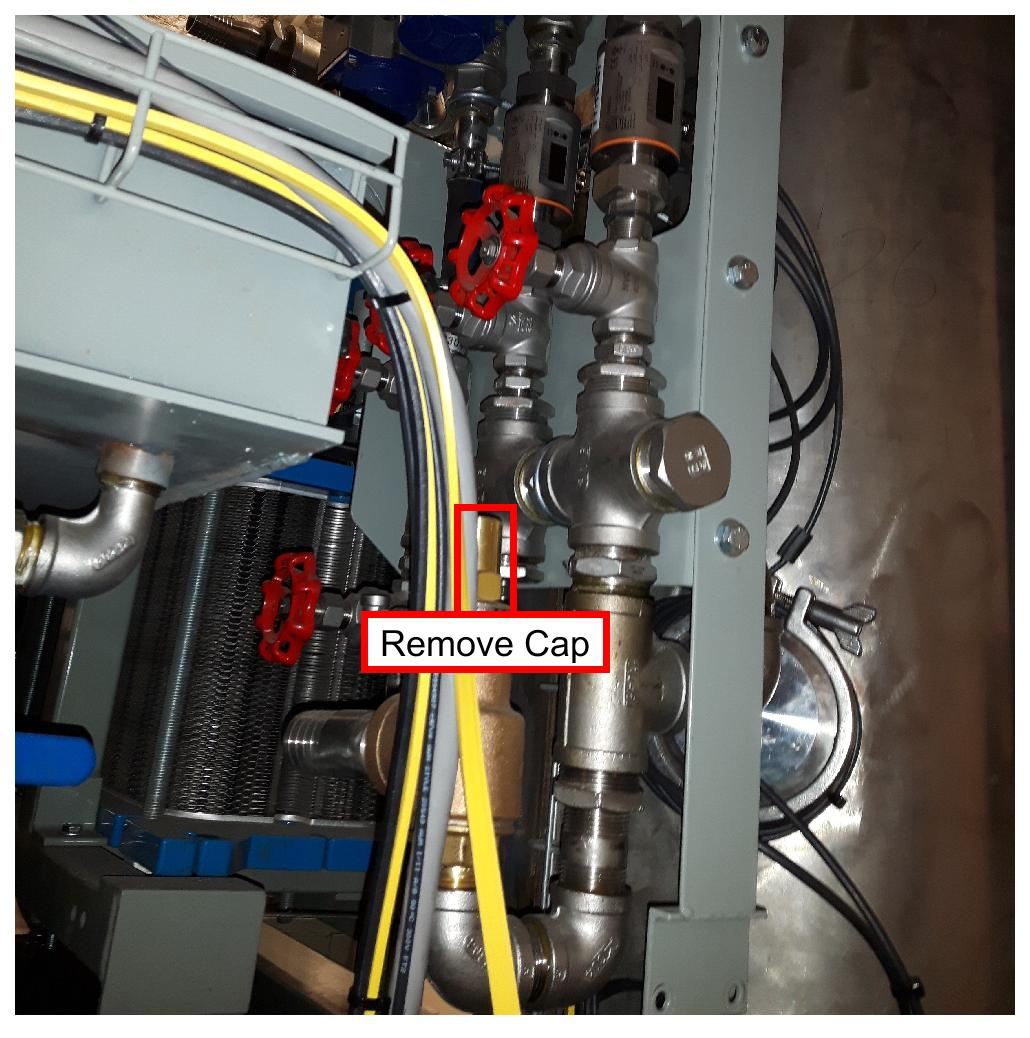
\includegraphics[width=0.45\textwidth]{pictures/filter_swap/prv_loc.jpg}
        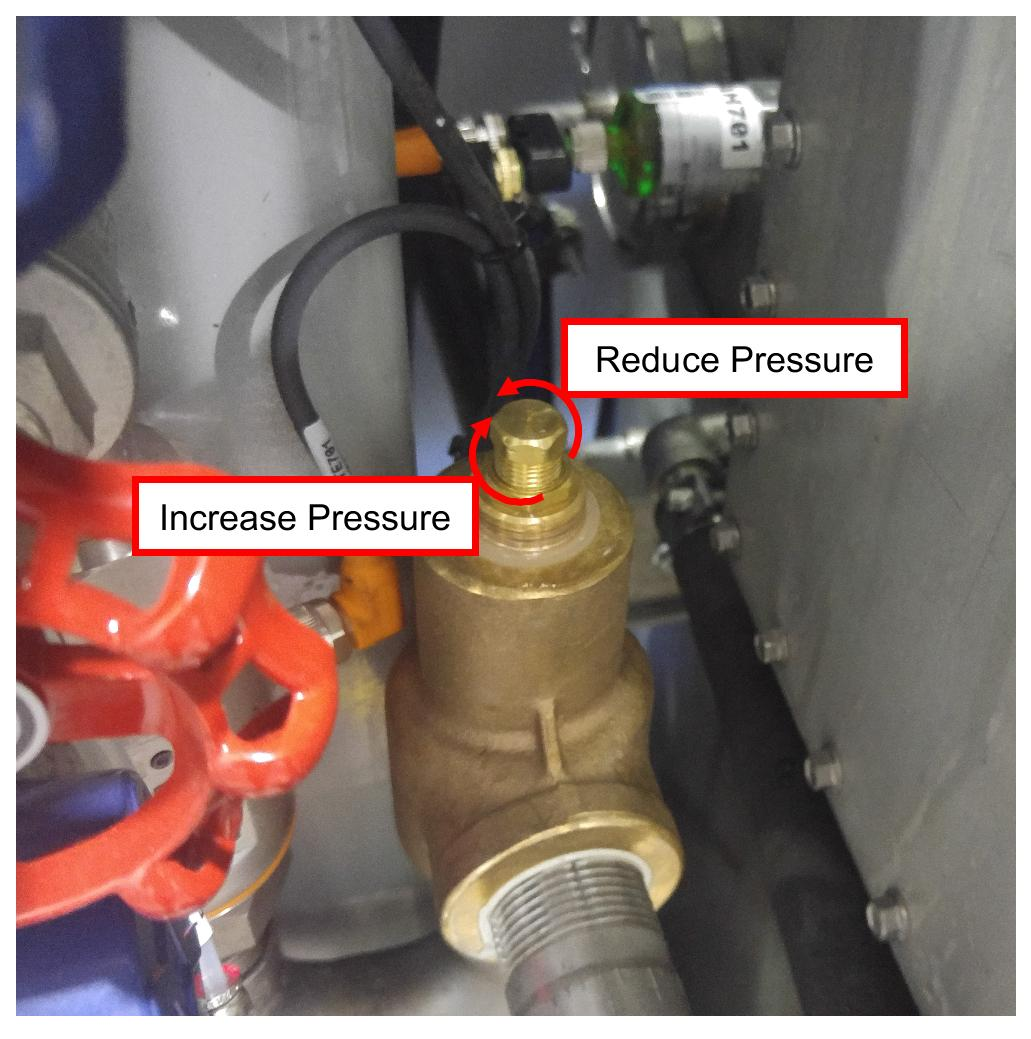
\includegraphics[width=0.45\textwidth]{pictures/filter_swap/prv_mech.jpg}
        \caption{Pressure Release Valve Adjustment}
        \label{fig:cab3_conn}
\end{figure}

Step 4: On the HMI, you should read the following values: PT503 = 20 psi and PT502 = 35 PSI.\\
\newpage
Step 5: Go to the settings page on the HMI and make sure the following settings have the values shown below:

\begin{itemize}
    \item Set\_Filter\_PT502\_NewFilter = 35 psi
    \item Set\_Filter\_PT502\_CloggedFilter = 46 psi
    \item Set\_PT502\_TrigDelay = 20 sec
    \item Set\_Filter\_PT503\_LowPressure = 10 psi
    \item Set\_Filter\_PT503\_LowPressure\_TrigDelay = 10 sec
\end{itemize}